\chapter[Arquitetura Proposta]{Arquitetura Proposta}
\label{cap:proposta}

Este capítulo descreve a arquitetura que constitui a contribuição central desta
tese. A descrição aqui apresentada corresponde ao sistema efetivamente implementado
e avaliado, cujos resultados são relatados no Capítulo~\ref{cap:resultados}.

\section{Delimitação do Escopo}
\label{sec:prop-escopo}

Convém delimitar, antes da descrição técnica, o que esta arquitetura se propõe a
resolver e o que deliberadamente deixa de fora.

\subsection{O Problema Atacado}

Robôs de inspeção de subestações tipicamente seguem uma patrulha fixa, sem adaptar o
percurso ao que percebem. Um controlador puramente reativo, no extremo oposto,
responde apenas a estímulos já dentro do alcance sensorial --- e, portanto, nada
garante que os sensores cheguem aonde os eventos ocorrem. A arquitetura proposta faz
a ponte entre esses dois regimes.

\subsection{Aspectos Não Abordados}
\label{sec:prop-nao-abordado}

A percepção é abstraída em \emph{eventos}: modalidade, intensidade e posição,
fornecidos sem incerteza associada. Trata-se de simplificação deliberada e
delimitada, apropriada a uma contribuição \emph{algorítmica}: ela isola o
comportamento de navegação e decisão do problema (ortogonal) de percepção e mantém a
avaliação reprodutível. Em consequência:

\begin{itemize}
    \item não se trata de detecção, classificação ou segmentação de anomalias a
    partir de fluxos brutos de sensores;
    \item a transformada de localização \texttt{map}$\rightarrow$\texttt{odom} é
    mantida fixa, de modo que o erro de localização não é modelado;
    \item falsos positivos, falsos negativos e persistência realista de eventos
    permanecem fora do estudo;
    \item não há validação em subestação física.
\end{itemize}

A Seção~\ref{sec:res-ruido} relaxa parcialmente a primeira dessas idealizações,
injetando ruído gaussiano sobre posição e intensidade percebidas, e mede o efeito.

\section{Visão Geral: Uma Arquitetura de Duas Camadas}
\label{sec:prop-visao}

O sistema separa a inspeção em duas camadas cooperantes
(Figura~\ref{fig:prop-arquitetura}).

Uma camada \emph{deliberativa} executa a patrulha de inspeção: visita uma sequência
de \textit{waypoints} ao redor dos equipamentos usando uma pilha de navegação padrão
--- Nav2 com controlador \textit{Model Predictive Path Integral} (MPPI). Interpreta-se
essa camada como \emph{sensoriamento ativo}: já que um agente puramente reativo só
responde a estímulos dentro do alcance, é necessário um mecanismo \emph{anterior} que
leve os sensores até onde os eventos possam ocorrer. A patrulha provê exatamente esse
posicionamento.

Uma camada \emph{reativa}, denominada \textsc{Stay Alert}, roda sobre a patrulha. Ela
é governada por um campo de atração--repulsão $\Phi$, que cresce quando um evento
sensorial saliente entra no alcance, conduzindo o robô a \emph{aproximar-se} de
pontos de interesse ($\Phi$ positivo --- por exemplo, um ponto quente térmico ou uma
descarga parcial) ou a \emph{afastar-se} do perigo ($\Phi$ negativo --- por exemplo,
uma zona de arco elétrico).

A camada \textsc{Stay Alert} \emph{não} substitui o planejador: enquanto $\Phi$ está
neutro o robô segue a patrulha; quando um evento se torna saliente, \textsc{Stay
Alert} preempta o \textit{waypoint} corrente, emite uma meta de navegação focada ---
uma pose de aproximação ou de recuo --- e devolve o controle à patrulha uma vez
tratado o evento. O que esse desacoplamento preserva é concreto e verificável: o
Nav2 permanece o único produtor de \texttt{/cmd\_vel}, e portanto o planejamento
global, a checagem de colisão contra o mapa de custos e a geração de trajetória
continuam inteiramente a cargo da pilha de navegação. A camada reativa altera
\emph{qual} meta é perseguida e \emph{quando}, nunca os comandos de velocidade. Não
se alega, com isso, qualquer garantia formal de evitação de colisão, de
\textit{liveness} ou de otimalidade: o Nav2/MPPI não as oferece, e trocar a meta em
tempo de execução não as criaria. A propriedade reivindicada é de arquitetura ---
a resposta reativa é acrescentada sem substituir a camada que dirige o robô ---,
e seu preço em afastamento e em completude está medido no
Capítulo~\ref{cap:resultados}.

\begin{figure}[htb]
\centering
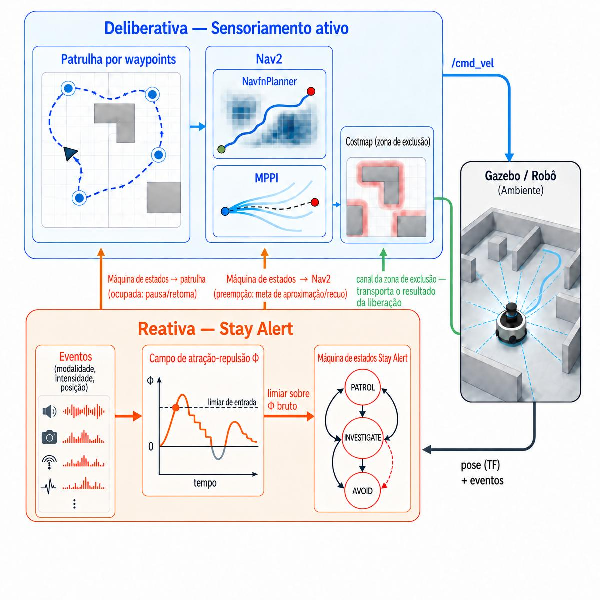
\includegraphics[width=0.9\textwidth]{figuras/architecture}
\caption{Arquitetura de duas camadas. A camada deliberativa (topo) conduz uma
patrulha por \textit{waypoints} através do Nav2 (NavfnPlanner $+$ MPPI), enviando
\texttt{/cmd\_vel} ao robô. A camada reativa (base, \textsc{Stay Alert}) converte
eventos percebidos no campo de atração/repulsão e executa a máquina de estados
finitos; ela preempta o Nav2 com uma meta de aproximação ou recuo e pausa ou retoma a
patrulha. O ambiente devolve pose (TF) e eventos.}
\label{fig:prop-arquitetura}
\end{figure}

\section{O Campo de Atração--Repulsão}
\label{sec:prop-campo}

A camada reativa é conduzida por um campo escalar $\Phi_t$ que agrega os eventos
sensoriais na localização do robô --- modalidade, intensidade e distância --- e
carrega o sinal da resposta: positivo para atração, negativo para repulsão. Ele é
função das observações correntes \emph{e} de duas memórias de canal com decaimento,
definidas adiante, de modo que é função do tempo, e não da observação instantânea
isolada. Ele não depende de qual ação é tomada. Escreve-se $\Phi$ por $\Phi_t$ onde o
índice temporal for dispensável:

\begin{equation}
\label{eq:prop-phi}
\Phi
\begin{cases}
> 0 & \text{atração (anomalia: aproximar)}\\
< 0 & \text{repulsão (risco: recuar)}\\
= 0 & \text{neutro (comportamento padrão de patrulha).}
\end{cases}
\end{equation}

\subsection{Intensidade Percebida e Fronteira de Detecção}

O campo é formado a partir de \emph{eventos} sensoriais. Um evento $e$ de modalidade
$m\in\{\text{térmica},\text{acústica},\text{risco}\}$ a uma distância $d$ do robô é
percebido dentro de um raio de detecção $R$ com intensidade

\begin{equation}
\label{eq:prop-intensidade}
i_e(d) = I_e\left(1 - \tfrac{1}{2}\,\frac{d}{R}\right), \qquad d \le R,
\end{equation}

sendo $I_e$ sua intensidade base. Esse perfil modela uma \emph{fronteira suave de
detecção}: o sensoriamento degrada linearmente com o alcance e não é reportado além
de $R$.

O degrau resultante em $d=R$ --- de $I_e/2$ para a ausência de evento --- é uma
descontinuidade real da intensidade percebida. Dois mecanismos do controlador
destinam-se a impedir que ela produza disparos repetidos: a histerese, com limiares
distintos de entrada e saída (Seção~\ref{sec:prop-stayalert}), e o compromisso, pois
uma vez comprometido um evento ele não é reselecionado até o fim do episódio.

\subsection{Canais com Memória e Precedência Categórica}

Cada modalidade possui um peso $w_m$ (com $w_{\text{risco}}<0$, para repulsão) e um
limiar de disparo $\theta_m$. O campo impõe \emph{segurança antes de inspeção} como
regra de \emph{precedência}, e não como disputa de magnitude: sempre que qualquer
evento repulsivo esteja acima do limiar e dentro do alcance, $\Phi$ assume seu valor
(negativo); apenas na ausência de risco o campo seleciona, entre os eventos de
atração concorrentes, o de maior magnitude.

Sejam $\mathcal{E}_{\mathcal{H}}$ e $\mathcal{E}_{\mathcal{A}}$ os conjuntos de
eventos de risco e de atração acima do limiar e dentro do alcance no passo corrente.
O evento governante e o campo são formados por \emph{dois acumuladores com
decaimento} --- um canal de risco $h\ge 0$ e um canal de atração com sinal $a$ ---
em vez de por uma única seleção instantânea. Escrevendo $c_e=w_{m(e)}\,i_e$ para a
contribuição com sinal do evento $e$, cada passo atualiza os canais por retenção de
máximo preservadora de magnitude:

\begin{align}
\label{eq:prop-canais}
h &\leftarrow \max\!\big(h,\ \textstyle\max_{e\in\mathcal{E}_{\mathcal{H}}}|c_e|\big),\\
a &\leftarrow c_{e^\star}\ \ \text{quando } |c_{e^\star}|>|a|\ \ (\text{retido, caso contrário}),
\end{align}

com $e^\star=\operatorname*{arg\,max}_{e\in\mathcal{E}_{\mathcal{A}}}|c_e|$ e empates
resolvidos pela menor identidade de evento. Uma vez por período de decaimento, ambos
os canais relaxam geometricamente e são zerados em um resíduo $\varepsilon$:

\begin{equation}
\label{eq:prop-decaimento}
h\leftarrow\lambda h,\qquad a\leftarrow\lambda a\quad(\text{zerado se abaixo de }\varepsilon).
\end{equation}

Cada acumulador é \emph{saturado no próprio lugar} na atualização ---
$h\in[0,\Phi_{\max}]$ e $a\in[-\Phi_{\max},\Phi_{\max}]$ ---, de modo que o valor
armazenado, e não apenas sua leitura, é limitado. O campo é então lido por
\emph{precedência categórica}:

\begin{equation}
\label{eq:prop-precedencia}
\Phi=-h\ \ \text{se } h>\varepsilon,\qquad
\Phi=a\ \ \text{caso contrário,}
\end{equation}

com decaimento $\lambda\in(0,1)$, resíduo $\varepsilon$ e período de decaimento
$T_d$. Quando o conjunto elegível \emph{próprio} de um canal está vazio em um passo,
esse canal é deixado ao decaimento da Equação~\eqref{eq:prop-decaimento} enquanto o
outro ainda pode ser atualizado por seus eventos.

Essa memória tem duas consequências que uma regra puramente instantânea não teria:

\begin{enumerate}
    \item um risco \emph{recentemente observado} continua governando o campo através
    de sua magnitude em decaimento, mesmo quando apenas uma atração está no alcance no
    passo corrente, até que $h$ caia abaixo de $\varepsilon$;
    \item um evento corrente mais fraco não sobrescreve um evento armazenado mais
    forte até que este último tenha decaído.
\end{enumerate}

Riscos são considerados primeiro, de sorte que um canal de risco acima de
$\varepsilon$ sempre governa o campo, independentemente de uma atração concorrente
mais forte: a disputa de magnitude decide apenas \emph{qual anomalia} aproximar,
nunca se preferir inspeção à segurança. Essa propriedade é verificada diretamente no
cenário de conflito da Seção~\ref{sec:res-conflito}.

\section{A Camada Reativa \textsc{Stay Alert}}
\label{sec:prop-stayalert}

A camada \textsc{Stay Alert} é uma máquina de estados finitos com três modos:
\textsc{Patrol}, \textsc{Investigate} (atração) e \textsc{Avoid} (repulsão),
sumarizados no Algoritmo~\ref{alg:stayalert} e na Figura~\ref{fig:prop-fsm}.

A repulsão tem prioridade sobre a atração --- segurança antes de inspeção --- a
partir de \emph{qualquer} estado: sempre que $\Phi \le -\theta_{\text{in}}$ e houver
pose de recuo disponível, o robô entra em \textsc{Avoid} e navega até a pose de
recuo, \emph{preemptando} uma \textsc{Investigate} em curso (desfecho
\emph{adiado}), sujeito a um curto período refratário $t_{\text{ref}}$ que impede
redisparo imediato enquanto a zona de exclusão deliberativa assume. Caso contrário, a
partir de \textsc{Patrol}, se $\Phi \ge \theta_{\text{in}}$ a camada compromete o
evento mais saliente no alcance e entra em \textsc{Investigate}, navegando até sua
pose de inspeção. Ao entrar em qualquer dos modos, a camada ativa uma marca de
\emph{ocupado} que pausa a patrulha e emite um marcador de evento com a identidade do
alvo.

\subsection{Controle e Crédito São Etapas Distintas}
\label{sec:prop-confirmacao}

Duas etapas devem ser mantidas separadas, porque somente a primeira atua sobre o
robô.

O \emph{controlador} encerra um episódio de \textsc{Investigate} quando a navegação
reativa \emph{tem sucesso} e esta se mantém por uma permanência comandada
$t_{\text{dwell}}$. Uma navegação abortada ou cancelada, ou o esgotamento de um
orçamento $t_{\max}$, encerra o episódio como \emph{falho}. Em qualquer das saídas
ele emite um evento com a identidade do alvo e o motivo.

O \emph{avaliador}, um nó separado, recebe esse evento e só então compara a pose do
robô com a posição \emph{verdadeira} do alvo: dentro de uma \emph{distância de
confirmação} --- a distância de parada acrescida de uma tolerância --- a anomalia é
creditada como \emph{inspecionada}; caso contrário, o episódio é registrado como
rejeição na confirmação.

A confirmação, portanto, jamais retroalimenta o comportamento: nenhum episódio é
prolongado ou abreviado por ela. É também uma aproximação: não se verifica
independentemente a distância de parada completa nem a orientação, tampouco a
persistência ao longo de toda a permanência, e a métrica é nomeada de acordo.

O episódio \emph{não} termina meramente porque $\Phi$ decaiu, o que previne oscilação
ao atravessar um ``vale'' de baixa saliência entre eventos. O modo \textsc{Avoid}
termina quando o risco deixa o alcance, $\Phi > -\theta_{\text{out}}$ (\emph{seguro}),
ou ao alcançar a pose de recuo (\emph{recuado}), e então arma o período refratário.

Uma anomalia é \emph{comprometida} no \emph{início} de sua investigação --- após o
que deixa de atrair, removendo a oscilação
\textsc{Patrol}$\leftrightarrow$\textsc{Investigate} que surge quando um
\textit{waypoint} fica próximo a uma anomalia --- e é contada como
\emph{inspecionada} apenas mediante chegada bem-sucedida confirmada. Episódios que
terminam como \emph{falho} ou \emph{adiado} são mantidos como desfechos distintos e
jamais contados como inspeções.

\subsection{A Zona de Exclusão Deliberativa}
\label{sec:prop-keepout}

Um risco \emph{sobre} a rota de patrulha não pode ser resolvido apenas por recuo
reativo, já que o \textit{waypoint} seguinte está além dele. Acrescenta-se, por isso,
uma expressão \emph{deliberativa} da repulsão: sempre que um risco é \emph{detectado}
dentro do alcance sensorial, sua posição \emph{percebida} é projetada como região de
exclusão \emph{persistente} no \textit{costmap} global, que o planejador então
contorna pelo restante da missão. Essa projeção é um canal de mapa acionado por
detecção --- não consequência de completar um recuo --- e usa a mesma informação
percebida que a camada reativa.

A entrega a esse canal é mais estreita do que ``suprimir $\Phi$'', e a distinção
importa. Ela ocorre na \emph{entrada} em \textsc{Avoid} e somente onde o canal de
exclusão está habilitado. O que ela bloqueia é a \emph{publicação} daquele risco como
evento: o risco deixa de ser reportado à camada reativa, de modo que novas
observações param de alimentar o acumulador de risco $h$. O valor já armazenado em
$h$ não é zerado --- ele decai pela Equação~\eqref{eq:prop-decaimento} até cair abaixo
de $\varepsilon$ --- e a região de exclusão permanece travada nesse meio-tempo, de
sorte que o planejador segue contornando a marca enquanto o sinal reativo se esvai. O
propósito é impedir que o robô oscile entre recuar e reaproximar enquanto o contorno é
percorrido.

Onde a zona de exclusão está \emph{desabilitada} --- o que ocorre em todo cenário fora
da rota --- não há entrega, o risco continua a ser publicado e a reobservação renova
$h$; a janela de supressão medida na Seção~\ref{sec:res-custo-precedencia} é,
portanto, mais longa do que o decaimento sozinho produziria.

\begin{figure}[htb]
\centering
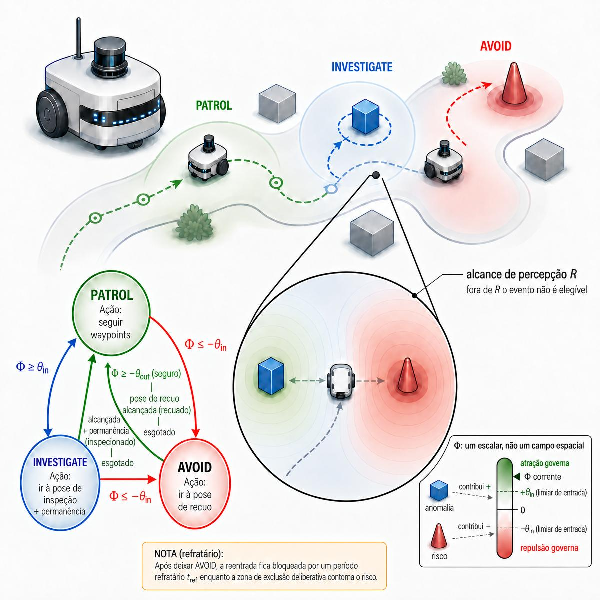
\includegraphics[width=0.9\textwidth]{figuras/stay_alert_fsm}
\caption{Máquina de estados \textsc{Stay Alert} e campo de atração--repulsão. Topo:
ao longo da patrulha o robô comuta para \textsc{Investigate} (aproximar-se de uma
anomalia) ou \textsc{Avoid} (recuar de um risco). Inferior esquerda: os três modos e
suas transições (limiares $\theta_{\text{in}},\theta_{\text{out}}$; desfechos
\emph{inspecionado}/\emph{esgotado}/\emph{seguro}/\emph{recuado}; a repulsão tem
prioridade). Inferior direita: o campo puxa em direção à atração e empurra para longe
da repulsão.}
\label{fig:prop-fsm}
\end{figure}

\begin{algorithm}[htb]
\caption{Camada reativa \textsc{Stay Alert} (por ciclo de controle)}
\label{alg:stayalert}
\begin{algorithmic}[1]
\STATE \textbf{entrada:} campo $\Phi$; evento selecionado $e^\star$ (mais saliente no
       alcance); limiares $\theta_{\text{in}},\theta_{\text{out}}$;
       $t_{\text{dwell}}, t_{\max}$; refratário $t_{\text{ref}}$
\STATE \textbf{Preempção de segurança} (um risco interrompe \emph{qualquer} estado):
\IF{o recuo reativo está habilitado \textbf{e} modo $\ne$ \textsc{Avoid}
    \textbf{e} $\Phi \le -\theta_{\text{in}}$
    \textbf{e} pose de recuo disponível \textbf{e} $t \ge t_{\text{avoid}}$}
  \IF{modo $=$ \textsc{Investigate}}
     \STATE sair (\emph{adiado por risco}); liberar alvo $e^\star$
  \ENDIF
  \STATE entrar em \textsc{Avoid}; pausar patrulha; enviar meta de recuo
  \IF{a zona de exclusão deliberativa está habilitada}
     \STATE \emph{entregar o risco à zona de exclusão}: cessar sua publicação à
            camada reativa, de modo que nenhuma nova observação alimente o canal de
            risco; o valor armazenado é mantido e deixado a decair
  \ENDIF
\ELSIF{modo $=$ \textsc{Patrol}}
  \IF{$\Phi \ge \theta_{\text{in}}$ \textbf{e} pose de inspeção disponível}
     \STATE comprometer alvo $e^\star$ (por identidade); entrar em
            \textsc{Investigate}; pausar patrulha; enviar meta de aproximação
  \ENDIF
\ELSIF{modo $=$ \textsc{Investigate}}
  \IF{navegação \textbf{bem-sucedida} \textbf{e} permanência $\ge t_{\text{dwell}}$}
     \STATE sair (\emph{inspecionado}); retomar patrulha
  \ELSIF{decorrido $\ge t_{\max}$ \textbf{ou} navegação abortada/cancelada}
     \STATE sair (\emph{falho}); retomar patrulha
  \ENDIF
\ELSIF{modo $=$ \textsc{Avoid}}
  \IF{$\Phi > -\theta_{\text{out}}$ \textbf{ou} pose de recuo alcançada}
     \STATE sair (\emph{seguro}/\emph{recuado});
            $t_{\text{avoid}} \gets t + t_{\text{ref}}$; retomar patrulha
  \ELSIF{decorrido $\ge t_{\max}$}
     \STATE sair (\emph{esgotado});
            $t_{\text{avoid}} \gets t + t_{\text{ref}}$; retomar patrulha
  \ENDIF
\ENDIF
\end{algorithmic}
\end{algorithm}

\section{Sensoriamento Ativo e Abstração de Eventos}
\label{sec:prop-sensoriamento}

A patrulha realiza o sensoriamento ativo ao conduzir os sensores ao longo da rota; a
pose do robô usada pela camada reativa é tomada no referencial do \emph{mapa} (via a
árvore TF), de modo que eventos, poses e o mapa estático sejam mutuamente
consistentes.

Dado um evento na posição $\bm{e}$ e o robô em $\bm{p}$, com direção unitária
$\hat{\bm{u}}=(\bm{p}-\bm{e})/\lVert\bm{p}-\bm{e}\rVert$, o modo
\textsc{Investigate} mira uma pose de inspeção a uma distância de parada $\rho$,
voltada para o evento,
$\bm{p}_{\text{insp}}=\bm{e}+\rho\,\hat{\bm{u}}$, enquanto \textsc{Avoid} mira uma
pose de recuo além do raio de detecção e voltada para o lado oposto,
$\bm{p}_{\text{ret}}=\bm{e}+(R+\Delta)\,\hat{\bm{u}}$. Eventos de atração são
comprometidos uma única vez, após o que deixam de atrair; riscos são persistentes.

\section{Sobre a Atualização de Valor}
\label{sec:prop-atualizacao}

O mesmo campo $\Phi$ pode ser escrito como termo adicional em uma atualização de
valor tabular, na forma

\begin{equation}
\label{eq:prop-bellman}
Q(s,a) \leftarrow Q(s,a) + \alpha\,\delta + \eta\,\Phi,
\end{equation}

sendo $\delta$ o erro de diferença temporal usual, $\alpha$ a taxa de aprendizado e
$\eta$ o peso do termo afetivo.

É preciso ser inequívoco quanto ao estatuto dessa formulação neste trabalho. A tabela
de valor \emph{não} seleciona as ações executadas: o comportamento imediato é
governado pelos limiares sobre o campo bruto $\Phi$ e pela máquina de estados do
Algoritmo~\ref{alg:stayalert}, e o movimento provém das metas enviadas ao Nav2/MPPI.
Em consequência, a varredura sobre $\eta$ relatada na literatura associada a este
trabalho constitui análise \emph{numérica da tabela de valor}, e não demonstração de
robustez comportamental --- e é assim que ela é apresentada.

%% Acrescentado em 12/11/2026. O estatuto teorico do termo aditivo precisa estar
%% declarado aqui, onde a equacao aparece, e nao so na conclusao: e a primeira coisa
%% que um leitor de aprendizado por reforco verifica.
Cabe ser igualmente inequívoco quanto ao estatuto \emph{teórico} do termo aditivo. O
campo $\Phi$ \emph{não} está formulado como termo potencial no sentido de
\citeonline{ng1999}, isto é, não assume a forma
$F(s,a,s')=\gamma\,\Phi(s')-\Phi(s)$ exigida para que a transformação preserve a
política ótima. O campo é aditivo, variante no tempo, sujeito a decaimento e
dependente dos eventos observados, de modo que \emph{nenhuma garantia de invariância
de política} se aplica à Equação~\eqref{eq:prop-bellman}, e nenhuma é reivindicada
nesta tese. Sob taxa de aprendizado $\alpha$ fixa, o incremento $\eta\Phi$ é,
ademais, representável como uma componente adicional de recompensa, à maneira de
outras abordagens que acoplam campos potenciais a aprendizado
\cite{zhang2023apf}: não há, portanto, novidade a reivindicar sobre o aumento de
recompensa no plano formal, e a contribuição desta tese não se localiza aí. Daí
também decorre a escolha de vocabulário mantida em todo o documento --- relata-se
\emph{estabilidade dos incrementos} nas simulações avaliadas, e não convergência.

Registra-se a formulação aqui como \emph{nota de projeto}, isto é, como caminho
previsto para uma política aprendida futura, e não como componente validado da
arquitetura avaliada. Para que esse caminho não ficasse apenas enunciado, ele foi
levado a funcionar em um braço separado: a Seção~\ref{sec:res-qdriven} relata um
\textit{baseline} em que uma tabela $Q$, treinada com recompensa aumentada por
$\Phi$, \emph{seleciona} a ação executada, medido contra o método nos três
cenários. O Capítulo~\ref{cap:resultados} relata o resíduo completo
$|\alpha\delta+\eta\Phi|$ como evidência de que os incrementos permanecem limitados
nas simulações avaliadas --- o que atesta estabilidade dos incrementos, e não
convergência, e muito menos que a atualização governe o comportamento.
